	% This template is taken from the following 
%       http://www-i6.informatik.rwth-aachen.de/~dreuw/latexbeamerposter.php
\documentclass[final]{beamer}

\newcommand {\cE} {\mathcal{E}}
\newcommand {\cD} {\mathcal{D}}
\newcommand{\E}{\ensuremath{\mathbb{E}} } %
\newcommand {\bxi} {\mbox{\boldmath $\xi$}}%
\newcommand{\bl}{\ensuremath{\mathbf{l}}} %
\newcommand{\bi}{\ensuremath{\mathbf{i}}} %
\newcommand{\bn}{\ensuremath{\mathbf{n}}} %
\newcommand{\bx}{\ensuremath{\mathbf{x}}} %

%\usepackage[absolute,overlay]{textpos}
%
%\setbeamercolor{framesource}{fg=gray}
%\setbeamerfont{framesource}{size=\tiny}
%\newcommand{\source}[1]{\begin{textblock*}{12cm}(1cm,8.6cm)
%    \begin{beamercolorbox}[ht=0.5cm,left]{framesource}
%        \usebeamerfont{framesource}\usebeamercolor[fg]{framesource} Source: {#1}
%    \end{beamercolorbox}
%\end{textblock*}}


\mode<presentation> {
        % you can chose your theme here:
	 %	\usetheme{Aachen} % black, orange, & ugly
		%  \usetheme{I6ac}
        % \usetheme{I6dv}        % the original
		 %  \usetheme{I6pd2}
        %  \usetheme{I6pd}
        %            \usetheme{Berlin}
        %               \usetheme[height=10cm]{Rochester}
        %               \usetheme{Madrid}
        %  \usetheme{I6pd2}
        %  \usetheme{I6td}
         \usetheme{Oldi6} % nice shade of blue in background
}

\graphicspath{{figures/}}

\usepackage{ragged2e, times, wrapfig, graphicx}
\usepackage{amsmath, amssymb, amsfonts, mathrsfs}
\usepackage{commath}
\usepackage{graphics,xcolor}
\usepackage[english]{babel}
\usepackage[latin1]{inputenc}
\usepackage[orientation=landscape,size=custom,width=121,height=91,scale=2,debug]{beamerposter}  % e.g. custom size poster

% - - - - - - - - - - - - - - - - - - - - - - - - - - - - - - - - - - - - - - -
        
        \title[Fancy Posters]{Minimum Time Control in SCARA Robot Simulation}
        \author{Sam Tormey, Nick Link, Rick LeVan. Advisor: Matthias Heinkenschloss}
        \institute{Department of Computational and Applied Mathematics, Rice University}
        
        
        
\begin{document} %%%%%%%%%%%%%%%%%%%%%%%%%%%%%%%%%%%%%%%%%%%%%%%%%%%%%%%%%%%%%%
        \begin{frame}{}
        
        \vfill
        \vspace{-1.5cm}
		%\vspace{0.5cm}
% =============================================================================
%                                     Column 1
% =============================================================================
{\footnotesize
\begin{columns}[t]
        
\hspace{0.7cm}
\begin{column}{.30\linewidth}
                
\begin{block}{\centering Introduction}
		

%\vspace{0.8cm}

\vspace{0.3cm}


\begin{itemize}
		\item Improving the efficiency of recycling through automation was the inspiration for our project.
	\item We model the removal of objects from a conveyor belt with a MATLAB simulation of a SCARA robot.

	\item We solve a constrained optimization problem to find the optimal path between starting and
ending configurations. 
\end{itemize}

\begin{columns}[T]
\begin{column}{16cm}{}
	\vspace{0.5cm}
	\centering \includegraphics[height=12cm, width = 14cm]{figures/mrf-recycling-system.jpg}\\
\end{column}
\begin{column}{16cm}{}
	\centering \includegraphics[height=12cm, width = 14cm]{figures/scara.jpg}\\
\end{column}

\end{columns}
 
\end{block}
                
%-*-*-*-*-*-*-*-*-*-*-*-*-*-*-*-*-*-*-*-*-*-*-*-*-*-*-*-*-*-*-*-*-*-*-*-*-*-*-*-*-*-*-*-*
                
%\vspace{1cm}

\begin{block}{\centering Operating Principle} 


\begin{columns}[T]
\begin{column}{16cm}{}
	\vspace{0.7cm}
\[ \scalebox{2.3}{$\frac{\partial E}{\partial \theta_j} - \frac{d}{dt}\frac{\partial E}{\partial \dot{\theta_j}} = u_j$}\]

\vspace{0.3cm}

\begin{itemize}
	\item where $u_j$ is the torque at joint $j$.
	\item The Euler-Lagrange equation constrains kinetic energy and thus the possible system states.
\end{itemize}
\end{column}
\begin{column}{16cm}{}
Double Pendulum
\centering\includegraphics[height=15cm, width = 15cm]{figures/double-pendulum.png}\\
\end{column}

\end{columns}

\end{block}

                
%-*-*-*-*-*-*-*-*-*-*-*-*-*-*-*-*-*-*-*-*-*-*-*-*-*-*-*-*-*-*-*-*-*-*-*-*-*-*-*-*-*-*-*-*
                
%\vspace{1cm}

\begin{block}{\centering The Optimization Problem}


\begin{columns}[T]

\begin{column}{10cm}{}

	\underline{Continuous Form}
\begin{align*}
\min  & \: \:T \\
\mbox{s.t. } & \frac{dx(t)}{dt} = f(x(t),u(t)) \\
& x(0) = x_0 \\
& x(T) = x_T \\
& t \in [0, T] \\
& \norm{u(t)}_{\infty} \leq M \\
\end{align*}



\end{column}

\begin{column}{12cm}{}

	\underline{Discrete Form}
\begin{align*}
\min  & \: \:T \\
	\mbox{s.t. } & \frac{x_{i+1}-x_i}{\Delta\tau} = Tf(x_i,u_i) \\
& x_1 = x_0 \\
& x_n = x_T \\
& 1 \leq i \leq n \\
& \norm{u_i}_{\infty} \leq M \\
\end{align*}
\end{column}

\end{columns}


\begin{columns}[T]

\begin{column}{10cm}{}

\begin{itemize}
\item $T$ = total time taken by path 
\item $t$ = time 
\item $x(t)$ = state at time $t$ 
\end{itemize}

\end{column}

\begin{column}{10cm}{}

\begin{itemize}
\item $u(t)$ = control at time $t$ 
\item $x_0$ = initial state
\item $x_{\scriptsize\mbox{T}}$ = end state
\item $M$ = bound on torque
\end{itemize} 

\end{column}

\end{columns}

\end{block}


%-*-*-*-*-*-*-*-*-*-*-*-*-*-*-*-*-*-*-*-*-*-*-*-*-*-*-*-*-*-*-*-*-*-*-*-*-*-*-*-*-*-*-*-*
                        

 \end{column}
%-*-*-*-*-*-*-*-*-*-*-*-*-*-*-*-*-*-*-*-*-*-*-*-*-*-*-*-*-*-*-*-*-*-*-*-*-*-*-*-*-*-*-*-*
                        
        
% =======================================================================
%                                     Column 2
% =======================================================================
        
\begin{column}{.30\linewidth}

\begin{block}{\centering Discretized Precomputation}

\centering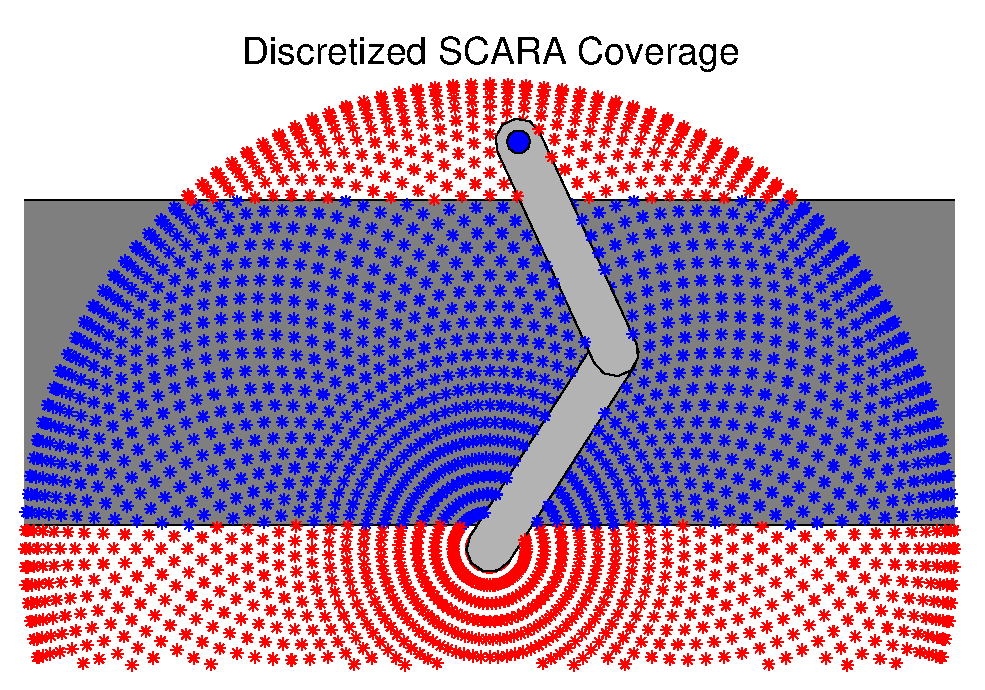
\includegraphics[height=22cm, width = 26cm]{figures/SCARA_coverage.eps}\\

\begin{itemize}

	\item The simulation needs to run efficiently in real time.
	\item Calls to fmincon are costly, however.
	\item To get around this, we precompute optimal paths between a fixed number of points.

\end{itemize}

%In order to run the simulation efficiently in real time, we precompute the optimal paths between a 
%finite number of goal regions and points on the belt. 


\end{block}
             

\begin{block}{\centering Optimizing the Optimization}



	%\vspace{-1cm}
\centering\includegraphics[height=30cm, width=30cm]{figures/Better6_Spy_Jacobian.eps} 



	\begin{itemize}
		\item We precompute the Jacobian matrix, where 2.67\% of entries are nonzero.
		\item This accelerates the fmincon solver.
	\end{itemize}
%To accelerate MATLAB's fmincon solver for our discretized optimization problem, we compute the
%Jacobian matrix



\end{block}

   

%-*-*-*-*-*-*-*-*-*-*-*-*-*-*-*-*-*-*-*-*-*-*-*-*untitled.eps-*-*-*-*-*-*-*-*-*-*-*-*-*-*-*-*-*-*-*-*               
%  \vspace{1cm}
                

 \end{column}
% =============================================================================
%                                     Column 3
% =============================================================================
        
\begin{column}{.30\linewidth}



                
\begin{block}{\centering Results}

	%\centering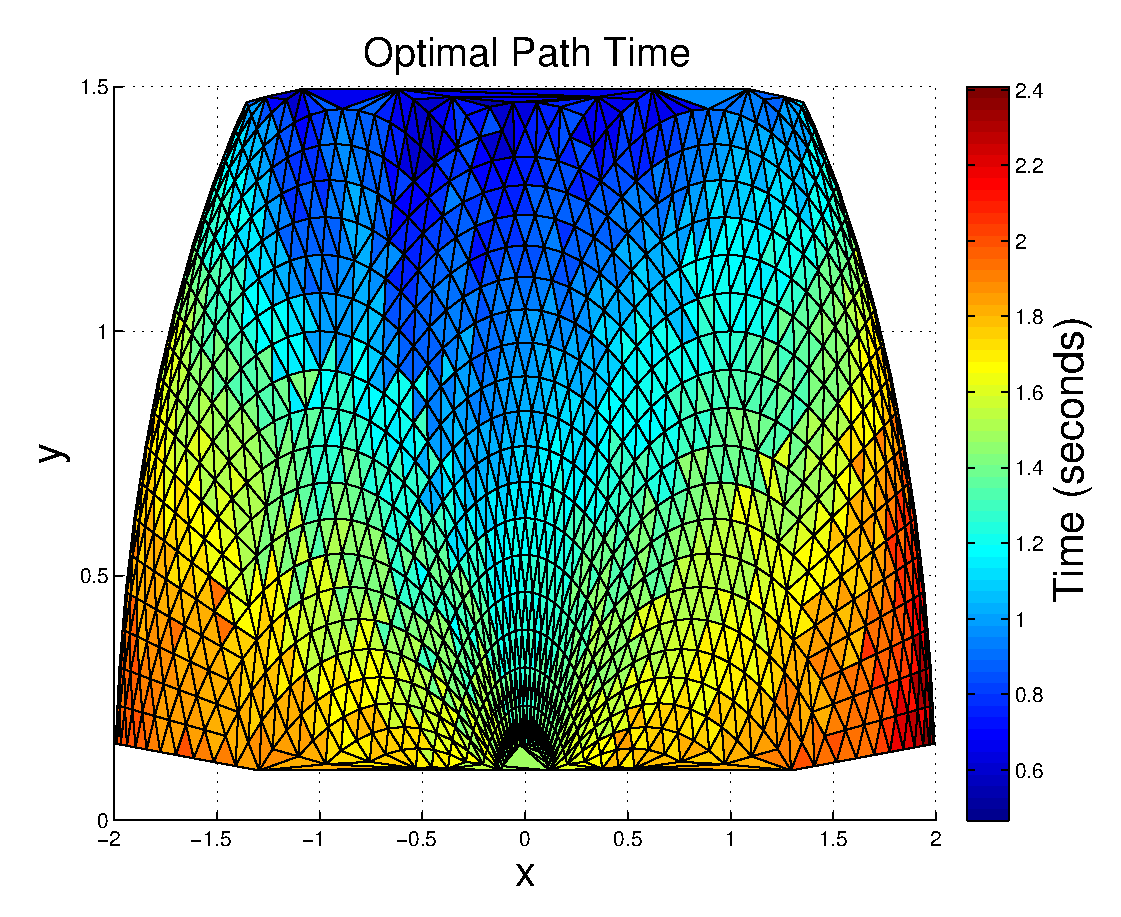
\includegraphics[height=30cm, width=30cm]{figures/Optimal_Path_Time.eps}
	\centering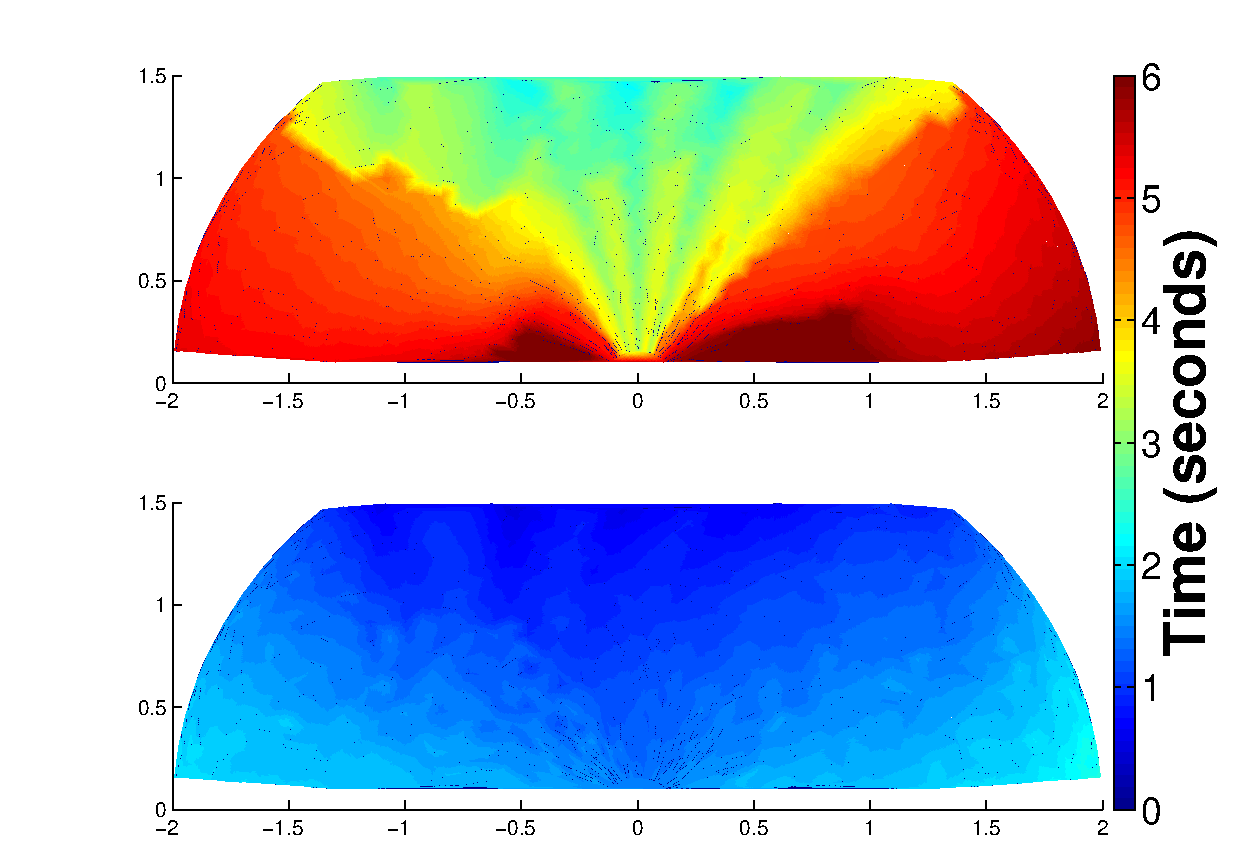
\includegraphics[height=25cm, width=25cm]{figures/MinTime_Controllers_vs_Optimal_Final.eps}

Variation in optimal time to reach a goal point given a starting robot configuration

\vspace{2cm}


\centering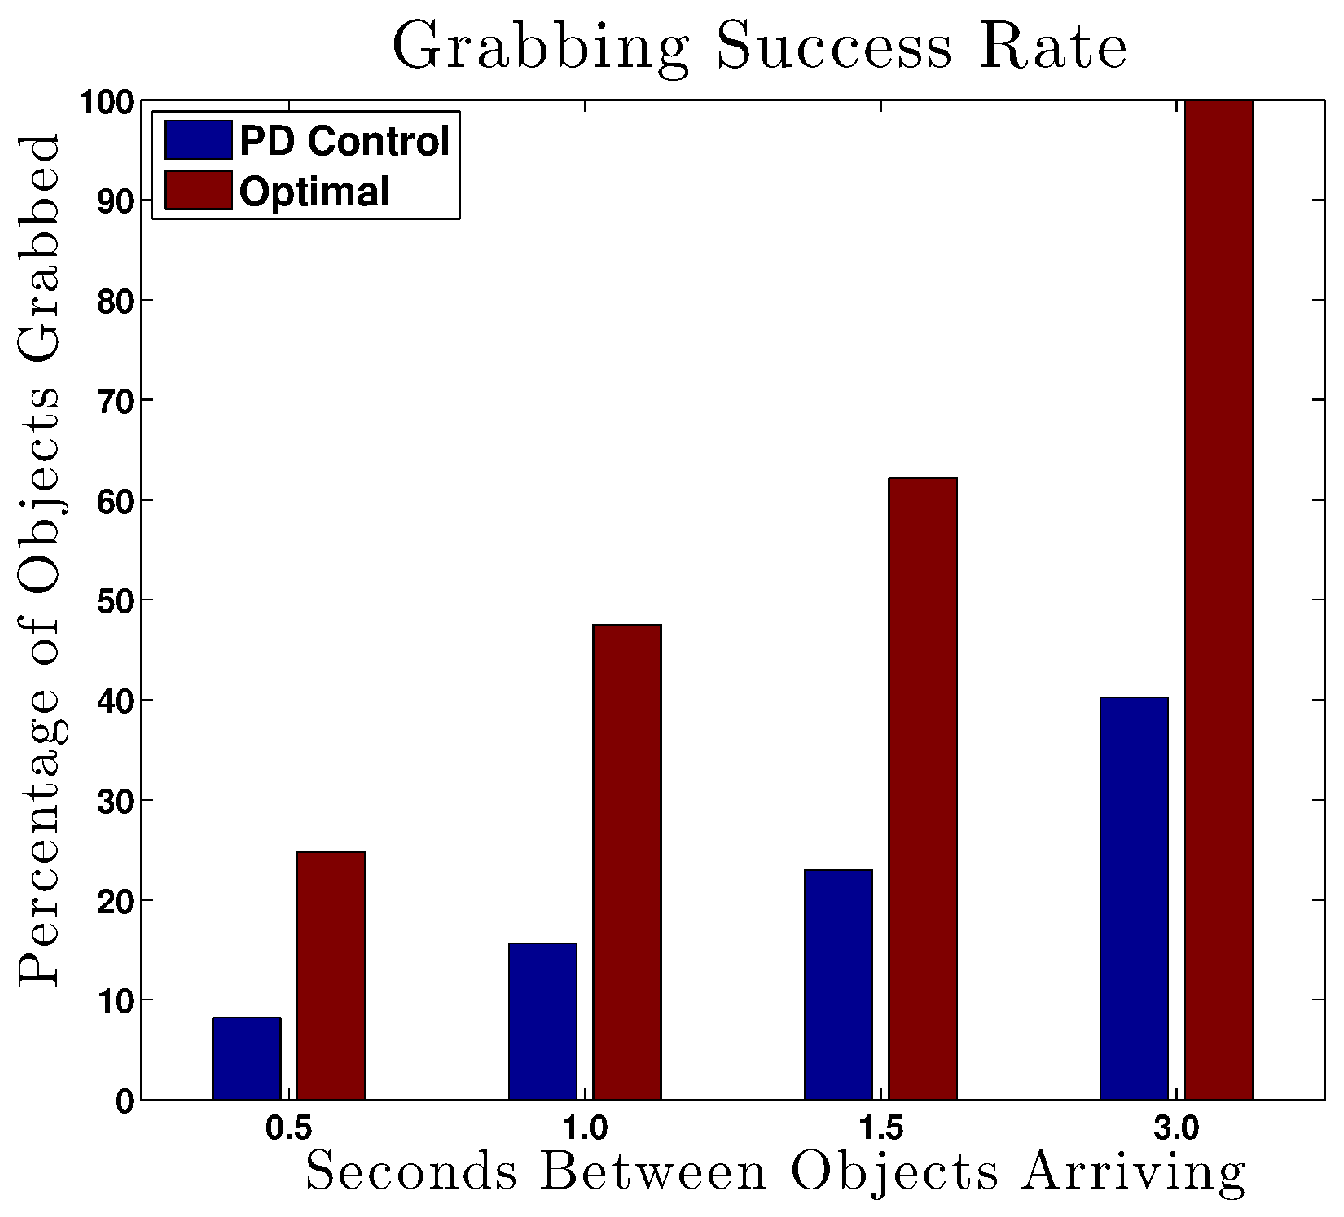
\includegraphics[height=28cm, width=30cm]{figures/bar_graph.eps}

\end{block}



                
%-*-*-*-*-*-*-*-*-*-*-*-*-*-*-*-*-*-*-*-*-*-*-*-*-*-*-*-*-*-*-*-*-*-*-*-*-*-*-*-*-*-*-*-*             
%  \vspace{1cm}
                
\begin{block}{\centering Future work}
\begin{itemize}
	\item Finding the reason for occasional failure of optimizing with MATLAB's fmincon.
	\item Investigating better ways of incorporating mod $2\pi$ arithmetic.
\end{itemize}
\end{block}
                
%-*-*-*-*-*-*-*-*-*-*-*-*-*-*-*-*-*-*-*-*-*-*-*-*-*-*-*-*-*-*-*-*-*-*-*-*-*-*-*-*-*-*-*-*                
% \vspace{0.5cm}
                
%                \setbeamertemplate{
%bibliography item}[text] % for numbering on the references

%               \begin{block}{References}
%                       \bibliographystyle{plain}
%                       \begin{thebibliography}{99}
                
                        %{\scriptsize \bibliography{refs}}
%\tiny \bibitem{SS} [1] F. Santosa and W. Symes, \textit{Linear Inversion of Band-Limited Reflection Seismograms,} 1986
%\tiny \bibitem{GRB} [2] Gurobi Optimization, \textit{Gurobi Optimizer Reference Manual,} 2012, \\ \url{www.gurobi.com}.
%\tiny \bibitem{RECPF} [3] J. Yang, Y. Zhang and W. Yin, \textit{A Fast Alternating Direction Method for TVL1-L2 signal reconstruction from Partial Fourier Data,} April 2010, \\
%\url{www.caam.rice.edu/~optimization/L1/RecPF/}.

                    
   %                 \end{thebibliography}
                       
                    
        %               \vspace{.05cm}
                %\end{block}
                
                %-*-*-*-*-*-*-*-*-*-*-*-*-*-*-*-*-*-*-*-*-*-*-*-*-*-*-*-*-*-*-*-*-*-*-*-*-*-*-*-*-*-*-*-*
                
%                \vspace{1cm}
                
%                \begin{block}{Aknowledgements}
%                
%                This work is partially funded by NSF Grant DMS-0811188 and DMS-1115950 and by CONACYT.
%                        %{\scriptsize
%        
%                                %\begin{figure}
%                                %\includegraphics{rice-logo} \hspace{1cm} 
%                                %\includegraphics{conacyt}\hspace{1cm} \includegraphics[width=2in]{nsf}
%                                %\end{figure}
%
%                                %  \center{ \tiny This work is partially funded by NSF Grant DMS-0811188 and DMS-1115950 and by CONACYT. }
%                        %}
%                \end{block}
                
\end{column}
        
\end{columns}
}       % end of footnotesize

\end{frame}
        
\end{document} %===================================================================================
%==================================================================================================
%%
%% \begin{block}{\large Fontsizes}
%%       \centering
%%       {\tiny tiny}\par
%%       {\scriptsize scriptsize}\par
%%       {\footnotesize footnotesize}\par
%%       {\normalsize normalsize}\par
%%       {\large large}\par
%%       {\Large Large}\par
%%       {\LARGE LARGE}\par
%%       {\veryHuge veryHuge}\par
%%       {\VeryHuge VeryHuge}\par
%%       {\VERYHuge VERYHuge}\par
%% \end{block}
%%
%%====================================================
%%
%%      \begin{block}{Methods}
%%              \begin{figure}[htbp]
%%                      \begin{center}
%%                              \includegraphics[width=7in]{lp_example2.pdf}
%%                              \label{ fig:lp_example1.pdf}
%%                      \end{center}
%%              \end{figure}
%%      \end{block}
%%
%%%%%%%%%%%%%%%%%%%%%%%%%%%%%%%%%%%%%%%%%%%%%%%%%%%%%%%%%%%%%%%%%%%%%%%%%%%%%%%%%%%%%%%%%%%%%%%%%%%%
%%% Local Variables: 
%%% mode: latex
%%% TeX-PDF-mode: t
